\chapter{Background and Motivation}

\section{SDN}
The idea of programmable networks has been around since the early 90s \cite{Campbell1999}. The approach responds to the inflexibility and nontransparency of traditional networking: forwarding devices, or switches, when deployed could only be upgraded or changed at great costs, often by completely replacing the unit in question. The advent of the internet brought more massive networks with strict uptime requirements and lead to costly upgrades slowly becoming unfeasible. Overcoming internet ossification became a priority \cite{Anderson2005}. SDN soon established itself as the main approach for programmable networks to tackle the issue.

SDN works by separating the routing logic from the hardware switches, effectively uncoupling the control and data layers. Control logic is centralized into a software-based controller and the switches can be programmed via a protocol. The controller takes over the different functions that a legacy switch would have implemented locally, such as firewalls. For an illustration, see Figure \ref{fig:SDN_Explanation}. Of these protocols, OpenFlow is currently the most widely used.  It is maintained by the Open Network Foundation and has released multiple versions of its protocol, from 1.0 \cite{OpenNetworkingFoundation2009} to 1.5.1 \cite{OpenNetworkingFoundation2015}.

\begin{figure}[h!]
  \centering
  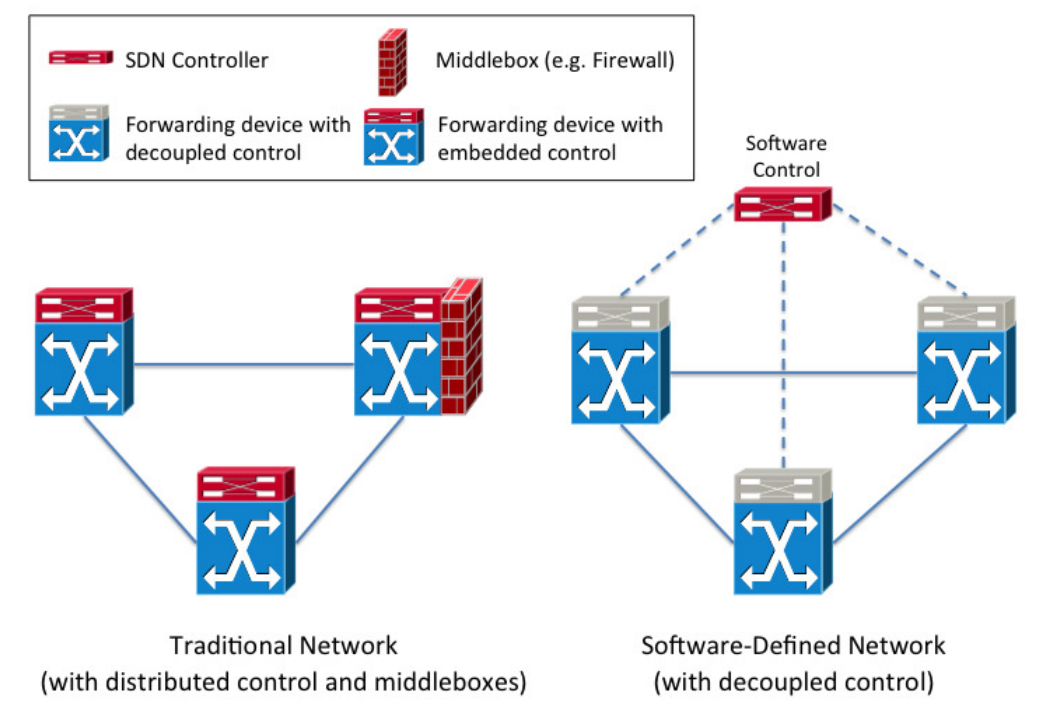
\includegraphics[scale=0.25]{SDN_Explanation.png}
  \caption{Comparison between legacy and SDN networks \cite{Nunes2014}}
  \label{fig:SDN_Explanation}
\end{figure}

Many benefits are promised by the widespread use of the SDN paradigm. Programmability in particular stands out: applications in the control layer can theoretically be developed with the freedom of any other piece of software without the need to overhaul the physical switches carrying out the forwarding instructions. Other benefits include ease of implementation and configuration \cite{Benzekki2016}. 

SDN's limitations, however, are also numerous. Centralization hampers scalability, for instance. Security concerns are much more acute than in legacy networks due to the increase in sensitive control traffic. Crucially, despite taking away the burden of control from the switches, SDN demands other types of performance from the hardware. The very installations researchers wanted to avoid having to upgrade suddenly need to cope with a very different set of requirements. This is the case for the space available in a flow table.

\subsection{Flow Rule Limitation}

The exploding size of routing tables is a phenomenon that long predates modern SDN. The internet, even in its infancy, was too complex a network for switches to naively route through, even with the advent of standards like CIDR \cite{TurnerJonathan;BianQiyong;Waldvogel1998}. This problem is exacerbated by the use of Ternary Content-Addressable Memories (TCAM) in Openflow-based SDN forwarding switches \cite{Luo2015}. TCAM allows ternary logic table look-ups that include a don't care bit value. Packets can be compared against an access list purely through hardware, making routing greatly efficient \cite{Hucaby2004}. Compared to their binary brethren however, TCAMs are significantly more expensive and consume more power, making their efficient use a priority \cite{ESiliconCorporation2014}.

When an OpenFlow-capable switch receives a packet it does not know how to route, it consults the controller for instructions. If the packet is to be routed and not dropped, a new entry is added to the rule table (or flow table, in OpenFlow parlance). There are three general approaches to combating the so-called flow table congestion problem: eviction, distribution and aggregation \cite{Leng2017}\cite{Nguyen2016}. 

Eviction-based methods seek to optimize the process by which flow table entries are removed from the flow table; in ideal circumstances they would only be evicted when they expire. Examples of such an approach include \cite{Vishnoi2014} and \cite{Lee2013}. Distribution, on the other hand, seeks to optimize the number of flow entries stored across the network and often copies or splits flows into multiple switches for that purpose \cite{Kanizo2013} \cite{Zhang2014}. 

The third major approach, aggregation (or compression) , is the one we are interested in for the scope of this research internship. 

\section{Flow Rule Aggregation}

The key difference between aggregation and other approaches is the preservation of the rule semantics in the switch. When observed from the outside, the switch behaves just as it would with an uncompressed rule table. It achieves this by finding groups of rules that can be covered with a single rule by virtue of their matches and actions. See Figure \ref{fig:AggregationIllustration} for an illustration. In contrast to eviction methods, no information is lost ahead of its allotted flow expiration time. Aggregation techniques can also be largely performed within the switch exclusively, with no need for controller-level knowledge of other parts of the network, as is the case for distribution methods.

\begin{figure}[h!]
  \centering
  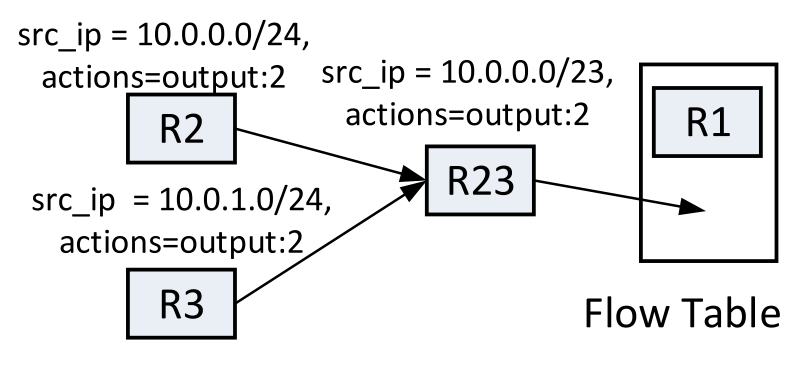
\includegraphics[scale=0.4]{AggregationIllustration.PNG}
  \caption{Example of flow rule aggregation \cite{Nguyen2016}}
  \label{fig:AggregationIllustration}
\end{figure}

POssibility of traditional IP compression techniques when adapted ???

Most compression techniques present an offline approach, meaning they have a clearly delimited update step in which the rules table is refreshed to compress as many rules as possible \cite{Leng2017}]. This update process is called with a certain regularity to keep the number of "superfluous" rules down. Some algorithms combine it with an online approach, in which small, gradual updates to the flow table are introduced to avoid long update steps \cite{Liu2010} \cite{Luo2014}. 


Aggregation techniques cause computational overhead. For offline techniques, reachability during the compression process can also lead to network instability. Additionally, flow rule granularity is purposefully reduced — by design visibility of individual flow rules is disregarded. Compression thus makes it impossible for the controller to control an aggregated flow without affecting the other rules involved. 

\section{Motivation for the Developed Platform}

Initially, the motivation behind this research internship was a more direct implementation and evaluation of different table rule compression algorithms. After analyzing the state of SDN and the existing code base at the chair, we pivoted towards a project that would more directly enable the research of flow table reduction techniques. 

OpenFlow provides a robust standard by which to implement Software-Defined Network principles and practice. The actual implementation of a controller and its applications, however, is left open. There are a number of controller implementations, in many of the most common programming languages, from open-source to proprietary \cite{Nunes2014}. A controller necessarily has abstract models of all the components of an SDN system, including switches, flow table entries, match fields, etc. This means that any given compression scheme could be implemented in a controller environment that successfully supports the OpenFlow standard.

The different controllers are mostly non-compatible — separate controller have no real reason to communicate with each other in classic SDN scenarios. This means that an aggregation algorithm implemented in a given controllers framework, could only work in that environment. The algorithm would need to be reimplemented from scratch should the controller change or the another system put in place. With no standard controller in the market, we identified the need for a platform that could enable the implementation and comparison of SDN Rule Aggregation Schemes regardless of the controller framework chosen. 

Additionally to controller platform-agnosticism, we strove to create a system which had the correct level of abstraction for the actual implementation of the individual elements to be independent of the functions they should fulfill. Easy extensibility, flexibility and modularity were our other guiding principles — new controllers and algorithms should be able to be implemented without overhauling other parts of the system.

An unavoidable choice was the 

Java - que es el unico constraint fuert porque eso es lo que ya existia en el sistema de la u

En el proximo capitulo estos van a ser nuestros guiding principles para la architectura